%-------------------------------------------------------------------------------
% Methoden
%-------------------------------------------------------------------------------
\section{Ergebnisse}
Im Folgenden werden die Ergebnisse des Experiments präsentiert.

\subsection{Beschreibung der Stichprobe}\label{beschreibung}
Das Experiment wurde am 05.07.2020 begonnen und endete am 11.09.2020. Bis zum 05.08.2020 kamen jedoch nur 39 Teilnehmende zusammen. Aus diesem Grund wurde zu diesem Zeitpunkt entschlossen, das Experiment auf Facebook und im Forum Hardwareluxx\footnote{www.hardwareluxx.de} zu teilen. Zusätzlich wurde das Experiment auf Reddit in dem Subreddit \textit{/r/takemysurvey/} und auf HackerNews\footnote{news.ycombinator.com/} beworben. Allerdings wurde die Studie als Eigenwerbung bewertet und nach wenigen Stunden auf HackerNews gelöscht. Da bis zum 05.09.2020 nach wie vor nicht ausreichend Personen an dem Experiment teilgenommen hatten, wurde die Studie erneut auf der Internetplattform HackerNews und zusätzlich durch Dr. rer. pol., Dipl.-Psych. Athanasios Mazarakis auf der Mensch und Computer 2020 (MuC) geteilt. Diese Kombination führte zu einem sprunghaften Anstieg der Teilnehmerzahlen. So kamen innerhalb von vier Tagen 141 neue Versuchspersonen hinzu.

Das Experiment war während der gesamten Dauer der Studie durchgehend erreichbar. In diesem Zeitraum nahmen insgesamt 279 Personen daran teil. Zunächst wurden 13 Einträge aus dem Datensatz entfernt, die für die folgenden Auswertung nicht berücksichtigt werden. Bei diesen Einträgen handelt es sich um Mehrfachteilnahmen, die sich durch identische IP-Adressen sowie identische User-Agents nachweisen ließen. In diesen Fällen wurde lediglich die erstmalige Teilnahme einbezogen; die nachfolgenden Einträge wurden aus dem Datensatz eliminiert. Zusätzlich wurden Einträge gelöscht, bei denen der Teilnehmende keinen Befehl abgeschickt hatte. Damit umfasst der bereinigte Datensatz 266 Teilnehmende. Davon haben 18 Personen das Experiment vollständig durchlaufen und sämtliche Fragen korrekt beantwortet.

Insgesamt gaben 210 Versuchspersonen an, männlich zu sein. Von den übrigen Versuchspersonen waren 28 weiblich und 27 Personen gaben ein anderes Geschlecht an. Der Großteil der Versuchspersonen verfügte, gemäß Selbsteinschätzung, über sehr gute (44 \%) oder gute (41 \%) Englischkenntnisse. 22 (8 \%) verfügten über schlechte Kenntnisse und 17 (6 \%) verfügten über keinerlei englische Sprachkenntnisse. Die Altersverteilung der Versuchspersonen stellt sich wie folgt dar: Insgesamt 100 Probanden waren 18-29 Jahre alt, 92  29-39 Jahre,  42 39-59 Jahre, 14 weniger als 18 Jahre und 18 gaben an, älter als 59 Jahre zu sein. Damit waren 88 \% der Versuchspersonen zwischen 18 und 59 Jahre alt. Ein Großteil davon nutzt die Kommandozeile mindestens einmal im Monat (46 \% täglich, 23 \% wöchentlich, 9 \% monatlich). Dagegen verwenden 11 \% die Kommandozeile selten (einmal im Jahr oder weniger) oder gar nicht (10 \%). Im Wesentlichen setzt sich die Stichprobe aus jungen und männlichen Versuchspersonen zusammen. Diese verfügen über gute Englischkenntnisse und können bereits erste Erfahrungen mit der Kommandozeile aufweisen.

\subsection{Deskriptive Statistik}
Im Mittel verbrachten die Versuchspersonen 527 Sekunden (SD = 1588) mit dem Experiment und setzten dabei durchschnittlich 19.5 Befehle ab (SD = 23.0). Eine besonders motivierte Versuchsperson investierte fast 5 Stunden in das Experiment und verwendete dabei 84 unterschiedliche Befehle. Keine andere Versuchsperson verbrachte mehr Zeit mit dem Experiment.

% Anzahl Befehle
\begin{figure}[htbp]
    \centering
    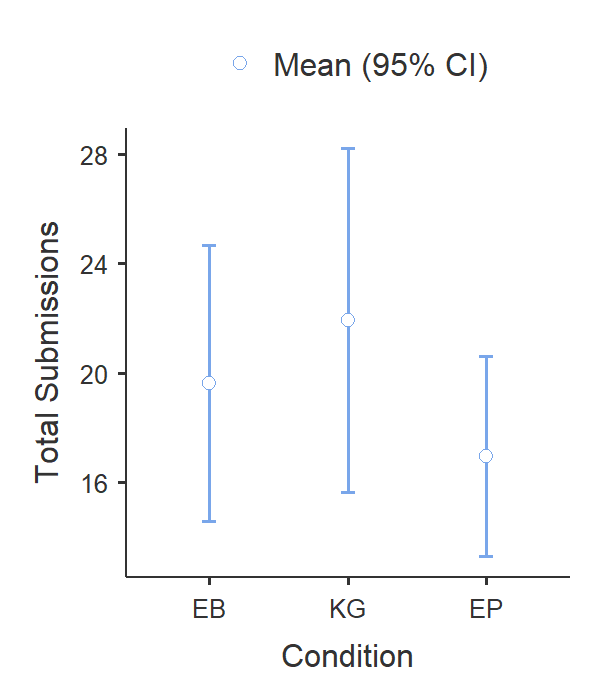
\includegraphics[width=0.5\textwidth]{img/auswertung/mean_subs.png}
    \caption{Mittelwerte der Gesamtzahl abgesetzter Befehle für die unterschiedlichen Versuchsbedingungen.}
    \label{mean_subs}
\end{figure}

Die Kontrollgruppe nutzte mit durchschnittlich 19.8 Befehlen die meisten Kommandos (SD = 26.7). Für die Versuchsbedingung mit Abzeichen wurde im Vergleich dazu eine durchschnittliche Anzahl abgesetzter Befehle von 18.4 (SD = 23.8) festgestellt, während Probanden aus der Bedingung mit Fortschrittsanzeige durchschnittlich 15.4 Befehle verwendeten (SD = 16.3). Die Mittelwerte und das zugehörige Konfidenzintervall sind in Abbildung \ref{mean_subs} dargestellt. Wird der Median der einzelnen Versuchsbedingungen betrachtet, stellt die Kontrollgruppe mit elf Kommandos pro Versuchsperson weiterhin die aktivste Bedingung dar. Allerdings sind Versuchspersonen der Experimentalgruppe mit Fortschrittsanzeige gemäß dem Median (10 Befehle) aktiver als Versuchspersonen, die ein Abzeichen erhielten (8.5 Befehle). Der Median der erfolgreich gelösten Aufgaben liegt bei den beiden Experimentalbedingungen bei drei Aufgaben und bei der Kontrollgruppe bei vier. Somit unterscheiden sich die drei Versuchsbedingungen hinsichtlich der Anzahl beantworteter Fragen und der dabei genutzten Konsolenbefehle nicht wesentlich voneinander. Auffällig ist die hohe Standardabweichung der genutzten Befehle in den einzelnen Bedingungen. Besonders die Gruppe mit Abzeichen und die Kontrollgruppe streuen stark um den Mittelwert und haben damit oft entweder deutlich mehr oder deutlich weniger mit der Anwendung interagiert, als es der Mittelwert vermuten lässt. Dies erklärt warum die Gruppe mit einer Fortschrittsanzeige im Mittel am wenigsten Befehle verwendete, aber nach dem Median mehr Befehle nutzte als bei der Versuchsbedingung mit Abzeichen. Bei der Fortschrittsanzeige liegen schlicht weniger Ausreißer vor.  

% Investierte Zeit
\begin{figure}[htbp]
    \centering
    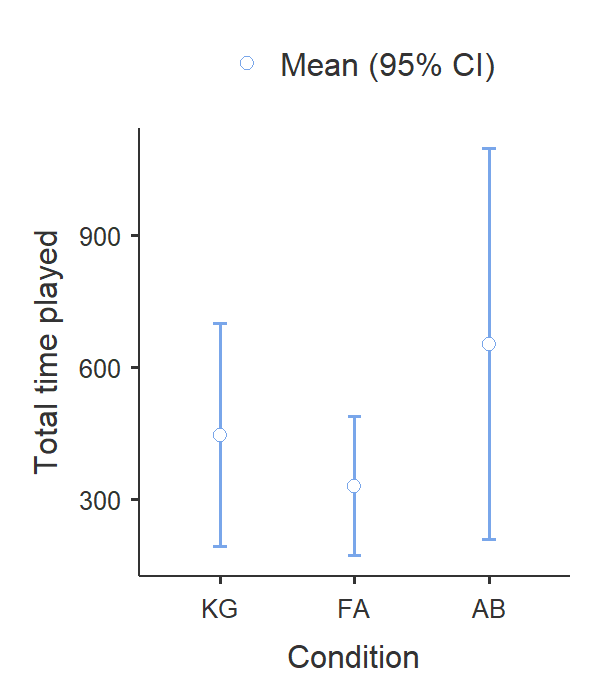
\includegraphics[width=0.5\textwidth]{img/auswertung/mean_time.png}
    \caption{Mittlere Gesamtspielzeit, die die unterschiedlichen Versuchsbedingungen in das Experiment investierten.}
    \label{mean_time}
\end{figure}

Im Bezug auf die Zeit, die die Teilnehmenden im Mittel in das Experiment investiert haben, fällt auf, dass die Teilnehmenden der Versuchsbedingung mit Abzeichen mit 654 Sekunden (SD = 2190) deutlich mehr Zeit investierten als die Kontrollgruppe (M = 447 Sekunden; SD = 1161 Sekunden). Letztere hat wiederum mehr Zeit mit dem Experiment verbracht als die Probanden der Versuchsbedingung mit Fortschrittsanzeige. Diese brachten 330 Sekunden (Standardabweichung 740) für das Experiment auf. Die entsprechenden Mittelwerte sind in Abbildung \ref{mean_time} dargestellt. Erneut zeigt sich eine, durch das große Streuungsintervall (siehe auch Abbildung \ref{mean_time}) induzierte, Verzerrung der Mittelwerte. Die jeweiligen Mediane für die unterschiedlichen Bedingungen liegen deutlich näher beieinander, als es der Durchschnitt erwarten lässt. Der Median der Kontrollgruppe liegt am höchsten (136), während die Gruppen Fortschrittsanzeige und Abzeichen nach dem Median weniger Zeit investierten (AB = 109; FA = 116). Bemerkenswert ist die hohe Abbruchquote in den ersten 30 Sekunden: 83 Versuchspersonen (31 \%) haben eine Gesamtspielzeit von unter einer halben Minute.

Aufgrund der hohen Diskrepanz zwischen Median und Mittelwert sowie der hohen Standardabweichung wurden extreme Ausreißer nicht in die weitere Betrachtung einbezogen. Bei diesen Ausreißern kann davon ausgegangen werden, dass eine, von den Spielelementen unabhängige, intrinsische Motivation vorliegt. Als Grenzwert wurde der Mittelwert zuzüglich der zweifachen Standardabweichung gewählt. Dies führt dazu, dass sämtliche Versuchspersonen mit mehr als 3537 Sekunden Spieldauer aus dem Datensatz ausgeschlossen wurden. Zusätzlich werden im Folgenden nur Teilnehmende berücksichtigt, die mindestens einen Befehl verwendet haben. Der so entstandene Datensatz hat einen Umfang von 240 Teilnehmenden (-26 ).

\subsection{Hypothesenüberprüfung}\label{hypo}
Die aufgestellten Hypothesen wurden durch einen t-Test und eine einfaktorielle  ANOVA  Varianzanalyse überprüft. Zunächst waren als Voraussetzungen die Normalverteilung und die Varianzhomogenität zu prüfen. Da jede Versuchsbedingung einen Umfang von deutlich über 30 Probanden aufweist, kann von einer Normalverteilung ausgegangen werden. Um die Voraussetzung der Varianzhomogenität zu prüfen, wurde ein Levene-Test durchgeführt. Dabei handelt es sich um einen Signifikanztest, durch den geprüft wird, ob die Varianzen innerhalb von zwei oder mehr Grundgesamtheiten (Gruppen) gleich sind (H0). Daraus ergibt sich die Alternativhypothese (H1), dass mindestens ein Gruppenpaar ungleiche Varianzen besitzt. Befindet sich der p-Wert unterhalb  eines zuvor definierten Signifikanzniveaus sind die Unterschiede in den Varianzen der unterschiedlichen Stichproben signifikant. Folglich kann die Nullhypothese des Tests abgelehnt und es kann angenommen werden, dass die Varianzen ungleich sind. Für die Auswertung wurde, wie allgemein üblich, ein Signifikanzniveau von 5 \% gewählt.

\subsubsection{Überprüfung mittels t-Test}

\paragraph{Hypothese 1 }
\begin{center}
    \textit{Probanden, die Abzeichen erhalten (AB), beantworten im Mittel eine höhere Anzahl an Fragen als eine Kontrollgruppe ohne Abzeichen (KG).} 
\end{center}

Der Levene-Test für die Anzahl an beantworteten Fragen ergibt mit  p = .318 kein  statistisch  signifikantes  Ergebnis (Levene-Statistik = 1.005). Bei der folgenden Untersuchung kann daher von Varianzhomogenität ausgegangen werden. Es ist keine Korrektur der Ergebnisse erforderlich. Die Differenz der durchschnittlichen Anzahl beantworteter Fragen von Probanden der Experimentalbedingung 'Abzeichen' und Probanden der Kontrollgruppe ohne Spielelemente ist nicht signifikant (t(160) = -1.118; p = .867). Die Hypothese kann damit nicht bestätigt werden. Daher wurde die ursprüngliche Hypothese abgewandelt und es wurden folgende Hypothesen aufgestellt:

\begin{itemize}
    \item \textbf{1.A:} \textit{Probanden, die Abzeichen erhalten (AB), verbringen im Mittel mehr Zeit mit dem Experiment als eine Kontrollgruppe (KG) ohne Spielelemente.}
    \item \textbf{1.B:} \textit{Probanden, die Abzeichen erhalten (AB), benutzen durchschnittlich mehr Befehle als eine Kontrollgruppe (KG) ohne Spielemente.} 
\end{itemize}

Für keine der zusätzlich aufgestellten Hypothesen ergibt sich ein auf dem 5\%-Niveau signifikanter p-Wert, weshalb erneut angenommen werden kann, dass die Varianzen der einzelnen Gruppen gleich sind. Die Ergebnisse des entsprechenden Levene-Tests sind in Tabelle \ref{levene_hypo_1} dargestellt. Folglich kann der unkorrigierte t-Test (Student's t) angewendet werden. Ein Vergleich  der  Mittelwerte  der Gesamtspielzeit der Kontrollgruppe mit der Gruppe mit Abzeichen führt nicht zu einem statistisch signifikanten Ergebnis (t(160) = 0.020; p = .492). Auch die durchschnittliche Anzahl an Befehlen unterscheidet sich bei den beiden Bedingungen nicht signifikant, t(160) = -0.570 , p = .715. Somit können weder Hypothese \textbf{H1} noch die abgewandelten Hypothesen \textbf{H1.A} und \textbf{H1.B} gestützt werden.


% ~*~*~*~*~*~*~*~*~*~*~*~*~*~*~*~ LEVENE - HYPO 1 ~*~*~*~*~*~*~*~*~*~*~*~*~*~*~*~
\begin{table}[htbp]
\centering
\caption{\textit{Levene-Test auf Varianzhomogenität für die Experimentalbedingung Abzeichen und die Kontrollgruppe (Hypothese 1).}}
\begin{tabular}{ p{4cm} p{2.0cm} p{2.0cm} p{2.0cm} p{2.0cm} }
 \hline
 & F & df1 &df2 &p \\
 \hline
  Befehlanzahl      & 0.044    & 1 &   160 & .834\\
  Gesamtspielzeit   & 0.110    & 1 &   160 & .741\\
  Gelöste Aufgaben  & 1.005    & 1 &   160 & .318\\
 \hline
 \multicolumn{5}{l}{%
 \small%
\textit{Anmerkungen}. * p < .05
}\\
\end{tabular}
\label{levene_hypo_1}
\end{table}
% ~*~*~*~*~*~*~*~*~*~*~*~*~*~*~*~ END ~*~*~*~*~*~*~*~*~*~*~*~*~*~*~*~
% ~*~*~*~*~*~*~*~*~*~*~*~*~*~*~*~ TEST - HYPO 1 ~*~*~*~*~*~*~*~*~*~*~*~*~*~*~*~
\begin{table}[htbp]
\centering
\caption{\textit{Zweistichproben-t-Test (Student's t) für die Experimentalbedingung Abzeichen und Kontrollgruppe (Hypothese 1).}}
\begin{tabular}{ p{4cm} p{2.0cm} p{2.0cm} p{2.0cm} }
 \hline
 & T &df & p \\
 \hline
  Befehlanzahl       & -0.570  &   160 & .715\\
  Gesamtspielzeit    &  0.020  &   160 & .492\\
  Gelöste Aufgaben   & -1.118  &   160 & .867\\
 \hline
 \multicolumn{4}{l}{%
 \small%
\textit{Anmerkungen}. $H_a:\: AB > KG$
}\\
\end{tabular}
\label{ttest_hypo_1}
\end{table}
% ~*~*~*~*~*~*~*~*~*~*~*~*~*~*~*~ END ~*~*~*~*~*~*~*~*~*~*~*~*~*~*~*~



\paragraph{Hypothese 2 }
\begin{center}
    \textit{Probanden, die eine Fortschrittsanzeige erhalten (FA), beantworten im Mittel eine höhere Anzahl an Fragen als eine Kontrollgruppe ohne Fortschrittsanzeige (KG).} 
\end{center}

Durch Levene-Test mit dem Ergebnis p = .806 bestätigt sich die Vermutung der Varianzhomogenität in den Gruppen. Mit t(150) = 0.373 und p = .355 ist die Differenz der durchschnittlichen Anzahl beantworteter Fragen bei Teilnehmenden der Experimentalbedingung mit Fortschrittsanzeige im Vergleich zu Versuchspersonen der Kontrollgruppe nicht signifikant. Die für Hypothese 1 abgewandelten Hypothesen wurden auch für die Versuchsbedingung mit Fortschrittsanzeige aufgestellt: 

\begin{itemize}
    \item \textbf{2.A:} \textit{Versuchspersonen, die eine Fortschrittsanzeige erhalten (FA), verbringen im Mittel mehr Zeit mit dem Experiment als eine Kontrollgruppe ohne Spielelemente (KG).}
    \item \textbf{2.B:} \textit{Versuchspersonen, die eine Fortschrittsanzeige erhalten (FA), benutzen durchschnittlich mehr Befehle als eine Kontrollgruppe ohne Spielelemente (KG).} 
\end{itemize}

 Wie zuvor sind die Varianzen in den Gruppen gleich, da der Levene-Test für keine der beiden Hypothesen signifikant ist (siehe Tabelle \ref{levene_hypo_2}). Ein durchgeführter t-Test führt bei einem Vergleich  der  Mittelwerte  der Gesamtspielzeit der Kontrollgruppe mit der Gruppe mit Fortschrittsanzeige nicht zu einem statistisch signifikanten Ergebnis (t(150) = 0.822; p = .794). Gleiches gilt für die Differenz zwischen den Mittelwerten der beiden Gruppen in Bezug auf die Anzahl der genutzten Befehle. Der entsprechende t-Test ist mit p = .137 nicht signifikant. Damit können Hypothese \textbf{H2} und die daraus abgeleiteten Hypothesen \textbf{H2.A} und \textbf{H2.B} nicht durch einen t-Test gestützt werden.


% ~*~*~*~*~*~*~*~*~*~*~*~*~*~*~*~ LEVENE - HYPO 2 ~*~*~*~*~*~*~*~*~*~*~*~*~*~*~*~
\begin{table}[htbp]
\centering
\caption{\textit{Levene-Test auf Varianzhomogenität für die Experimentalbedingung Fortschrittsanzeige und die Kontrollgruppe (Hypothese 2).}}
\begin{tabular}{ p{4cm} p{2.0cm} p{2.0cm} p{2.0cm} p{2.0cm} }
 \hline
 & F & df1 &df2 &p \\
 \hline
  Befehlanzahl      & 2.114     & 1 &   150 & .148\\
  Gesamtspielzeit   & 1.291     & 1 &   150 & .258\\
  Gelöste Aufgaben  & 0.061     & 1 &   150 & .806\\
 \hline
  \multicolumn{5}{l}{%
 \small%
\textit{Anmerkungen}. * p < .05
}\\
\end{tabular}
\label{levene_hypo_2}
\end{table}
% ~*~*~*~*~*~*~*~*~*~*~*~*~*~*~*~ END ~*~*~*~*~*~*~*~*~*~*~*~*~*~*~*~

% ~*~*~*~*~*~*~*~*~*~*~*~*~*~*~*~ TEST - HYPO 2 ~*~*~*~*~*~*~*~*~*~*~*~*~*~*~*~
\begin{table}[htbp]
\centering
\caption{\textit{Zweistichproben-t-Test (Student's t) für die Experimentalbedingung Abzeichen und Kontrollgruppe (Hypothese 1).}}
\begin{tabular}{  p{4cm} p{2.0cm} p{2.0cm} p{2.0cm}  }
 \hline
 & T &df & p \\
 \hline
  Befehlanzahl       & 1.099   &   150 & .863\\
  Gesamtspielzeit    & 0.822   &   150 & .794\\
  Gelöste Aufgaben   & 0.373   &   150 & .645\\
 \hline
 \multicolumn{4}{l}{%
 \small%
\textit{Anmerkungen}. $H_a:\: FA > KG$
}\\
\end{tabular}
\label{ttest_hypo_2}
\end{table}
% ~*~*~*~*~*~*~*~*~*~*~*~*~*~*~*~ END ~*~*~*~*~*~*~*~*~*~*~*~*~*~*~*~



% ~*~*~*~*~*~*~*~*~*~*~*~*~*~*~*~ ANOVA ~*~*~*~*~*~*~*~*~*~*~*~*~*~*~*~


\subsubsection{Überprüfung mittels ANOVA Varianzanalyse }
Bei der ANOVA (engl. \textit{Analysis of Variance}) handelt es sich um eine Varianzanalyse, anhand derer die Mittelwerte von mehr als zwei Gruppen verglichen werden können. Sie stellt eine Erweiterung des t-Tests dar, der auf den Vergleich von maximal zwei Stichproben beschenkt ist. Dies ermöglicht in diesem Fall den Vergleich aller drei Versuchsbedingungen. Nachfolgend werden die zwei abhängigen Variablen \textbf{Gelöste Aufgaben} und \textbf{Gesamtspielzeit} jeweils durch eine einfaktorielle Varianzanalyse untersucht.

% Varianzhomogenität prüfen 
Da ein Levene-Test sowohl für die Anzahl der gelösten Aufgaben (p = .606) als auch für die Gesamtspielzeit (p = .288) kein signifikantes Ergebnis ergibt, kann von Varianzhomogenität in den Gruppen ausgegangen werden. Eine nachträgliche Korrektur der Ergebnisse ist entsprechend nicht erforderlich. Die Varianzanalyse zeigt keinen statistisch signifikanten Unterschied im Zusammenhang der gelösten Aufgaben zwischen den einzelnen Versuchsbedingungen, F (2.237) = 0.626; p = .536. Selbiges gilt für die Gesamtspielzeit: Die Varianzanalyse zeigt zudem keinen statistisch  signifikanten Unterschied zwischen den einzelnen Versuchsbedinungen hinsichtlich der Spielzeit,  F(2.237) = 0.453, p = .636.


% ~*~*~*~*~*~*~*~*~*~*~*~*~*~*~*~ END ~*~*~*~*~*~*~*~*~*~*~*~*~*~*~*~

\subsection{Zwischenfazit t-Test und ANOVA}
Die geschilderten Ergebnisse entsprechen nicht den ursprünglichen Erwartungen. Tatsächlich kann weder durch einen t-Test noch durch eine ANOVA ein signifikanter Effekt in Bezug auf die Anzahl gelöster Aufgaben, die Menge der abgesetzten Befehle oder die Gesamtspielzeit nachgewiesen werden. Als Konsequenz wird keine der ursprünglich aufgestellten Hypothesen bestätigt. Die Spielelemente Abzeichen und Fortschrittsbalken zeigen durch das vorliegende Experiment keinen statisch signifikanten, positiven Effekt in Bezug auf das Durchhaltevermögen (gemessen anhand der Gesamtspielzeit). Auch lässt sich keine erhöhte Aktivität der Probanden feststellen, da sich die Versuchsbedingungen hinsichtlich der gelösten Aufgaben und der abgesetzten Befehle nicht signifikant unterscheiden. Stattdessen kann im Fall der Fortschrittsanzeige ein tendenziell negativer Einfluss beobachtet werden. Dieser zeigt sich insbesondere in der Gesamtspielzeit, die im Mittel deutlich geringer ist als bei den Alternativbedingungen. 

% ~*~*~*~*~*~*~*~*~*~*~*~*~*~*~*~ Weiterführende Analyse ~*~*~*~*~*~*~*~*~*~*~*~*~*~*~*~
\subsection{Weiterführende Analyse}
Um die Daten nachzuvollziehen und die Ergebnisse erklärbar zu machen, wurden sie ausführlicher untersucht: Der Verlauf des Experiments kann zeitlich in zwei Abschnitte unterteilt werden (siehe Abschnitt \ref{beschreibung}). Da anzunehmen ist, dass ab dem 06.09.2020 sehr versierte Versuchspersonen, die bereits Erfahrung mit der Kommandozeile haben, an dem Experiment teilnahmen, wurde beschlossen, das Experiment zeitlich in zwei disjunkte Abschnitte zu unterteilen. Dazu wurde der Datensatz in einen Abschnitt vor dem 06.09.2020 und einen Abschnitt ab dem 06.09.2020 aufgeteilt. Der erste Abschnitt besteht damit aus Versuchspersonen, die bis zum 05.09.2020 um 23:59:59 am Experiment teilgenommen haben, und die nachfolgend als \textbf{Gruppe 1} bezeichnet werden. Entsprechend setzt sich die andere Hälfte aus Versuchspersonen zusammen, die ab dem 06.09.2020 00:00 Uhr teilnahmen, und die \textbf{Gruppe 2} bilden. Teilnehmende ohne Interaktion (keine abgeschickten Befehle) werden erneut nicht berücksichtigt.

\subsubsection{Weiterführende Analyse - Zusammensetzung der Gruppen}
Zunächst wurden die demographischen Daten der beiden Gruppen miteinander verglichen. Die vollständige Gegenüberstellung ist in Tabelle \ref{demo_g12} dargestellt. Beide Stichproben setzen sich zu einem Großteil aus männlichen Probanden zusammen (> 80 \%). Die weiblichen und die diversen Teilnehmenden verteilen sich in den beiden Gruppen in gegensätzlicher Weise. So sind 13 \% der Teilnehmenden in Gruppe 1 weiblich und 6\% divers, während in Gruppe 2 6 \% weibliche und 14\% diverse Personen teilnahmen. Gruppe 1 verfügt durchschnittlich über weniger gute Englischkenntnisse als Gruppe 2 (35 \% vs 52 \% sehr gut). Gleichzeitig ist der Altersdurchschnitt in Gruppe 2 höher als in Gruppe 1. So ist der Großteil der Probanden aus Gruppe 2 zwischen 20 und 39 Jahre alt (39 \%). Demgegenüber gaben die Teilnehmenden der ersten Gruppe überwiegend ein Alter zwischen 18 und 29 Jahren an (49\%). Die Probanden aus Gruppe 2 nutzen die Kommandozeile zudem deutlich häufiger. Beispielsweise sind 66 \% der Probanden aus Gruppe 2  täglich mit dem Terminal befasst, während dies in Gruppe 1 lediglich auf 29 \% zutrifft. Damit ergeben sich die folgenden Profile für den jeweiligen Versuchsabschnitt:

Gruppe 1 setzt sich aus jungen, überwiegend männlichen Teilnehmenden zusammen, die über gute Englischkenntnisse verfügen und bereits erste Erfahrungen mit der Kommandozeile haben. 

Gruppe 2 setzt sich aus überwiegend männlichen Teilnehmenden mittleren Alters zusammen, die über gute bis sehr gute Englischkenntnisse verfügen und die die Kommandozeile häufig nutzen. 

% ~*~*~*~*~*~*~*~*~*~*~*~*~*~*~*~ Vergleich Demographie ~*~*~*~*~*~*~*~*~*~*~*~*~*~*~*~
\begin{table}[htbp]
\centering
\caption{\textit{Vergleich Demographie zwischen Gruppe 1 und Gruppe 2}}
\begin{tabular}{  p{6cm} p{3cm} p{3cm}  }
  \hline
  Merkmal & Gruppe 1 & Gruppe 2 \\
  \hline
  Umfang (absolut) & 121  & 123 \\
  \hline
  \multicolumn{3}{c}{Geschlecht} \\
  \hline
  Weiblich                      & 12.5 \%       & 5.7  \%       \\
  Männlich                      & 81.7 \%       & 80.5 \%       \\
  Divers                        & 5.8  \%       & 13.8 \%       \\
  \hline
  \multicolumn{3}{c}{Englischkenntnisse} \\
  \hline
  Sehr gut                      & 34.7 \%       & 52.0 \%      \\
  Gut                           & 48.8 \%       & 35.0 \%       \\
  Nicht so gut                  & 11.6 \%       & 6.5 \%        \\
  Nicht vorhanden               & 5.0  \%       & 6.5 \%        \\
  \hline
  \multicolumn{3}{c}{Alter} \\
  \hline
  <18                           & 6.6  \%       & 3.3  \%       \\
  18-29                         & 48.8 \%       & 27.6 \%       \\
  29-39                         & 32.2 \%       & 39.0 \%       \\
  39-59                         & 9.1  \%       & 22.0 \%       \\
  59+                           & 3.3  \%       & 8.1 \%        \\
  \hline
  \multicolumn{3}{c}{Häufigkeit der Nutzung der Kommandozeile} \\
  \hline
  Täglich (1x pro Tag)          & 28.9 \%       & 65.9  \%      \\
  Gelegentlich (1x pro Woche)   & 34.7 \%       & 13.8  \%      \\
  Selten (1x pro Monat)         & 11.6 \%       & 7.3  \%       \\
  Sehr selten (1x pro Jahr)     & 17.4 \%       & 4.9  \%       \\
  Nie                           & 7.4  \%       & 8.1  \%       \\
  \hline
\end{tabular}
\label{demo_g12}
\end{table}
% ~*~*~*~*~*~*~*~*~*~*~*~*~*~*~*~ END ~*~*~*~*~*~*~*~*~*~*~*~*~*~*~*~

\subsubsection{Weiterführende Analyse - Hypothesenprüfung}


Anschließend wurden die beiden Gruppen gesondert untersucht und analysiert. Wie zuvor wurden extreme Ausreißer sowie Versuchspersonen ohne Interaktion (kein Befehl gesendet) aus den Datensätzen eliminiert. Der jeweilige Grenzwert ergibt sich erneut aus dem Mittelwert zuzüglich der zweifachen Standardabweichung. In der Stichprobe, soweit sie zum 06.09.2020 zustande gekommen ist, liegt der Grenzwert der Spielzeit bei 5089 Sekunden. Teilnehmende, deren Gesamtspielzeit diesen Grenzwert übersteigt, wurden nachfolgend nicht berücksichtigt. Der so entstandene Datensatz hat einen Umfang von 117 Personen. Der entsprechende Schwellwert lag im Fall der zweiten Gruppe bei 1360 Sekunden. Dies führte zu einer Stichprobengröße von 116 Personen. Ziel des Vorgehens war es, die aufgestellten und in Abschnitt \ref{hypo} angepassten Hypothesen für die jeweilige Gruppe zu prüfen. Dabei wurden für jede Gruppe folgende Hypothesen betrachtet:

\paragraph{Hypothese 1}
\begin{itemize}
    \item \textbf{1.A:} \textit{Probanden, die Abzeichen erhalten (AB), verbringen im Mittel mehr Zeit mit dem Experiment als eine Kontrollgruppe (KG) ohne Spielelemente.}
    \item \textbf{1.B:} \textit{Probanden, die Abzeichen erhalten (AB), senden im Mittel mehr Befehle ab, als eine Kontrollgruppe (KG).}
    \item \textbf{1.C:} \textit{Probanden der Experimentalbedingung 'Abzeichen' (AB) lösen mehr Aufgaben als Personen der Kontrollgruppe.} 
\end{itemize}

\paragraph{Gruppe 1}
Die Werte für die Experimentalbedingung mit Abzeichen unterschieden sich mit $ t(71)=-0.325 $ und $p=.746$ nicht signifikant von der Kontrollgruppe hinsichtlich der absoluten Anzahl der genutzten Befehle. Auch für die durchschnittliche Spielzeit bei Personen, die ein Abzeichen erhielten, zeigt sich im Vergleich zur Kontrollgruppe kein signifikanter Unterschied ($t(71)=-0.396; p=.696$). Das Gleiche gilt für die Aufgabenzahl. Das Spielelement Abzeichen führte zu keinem signifikanten Unterschied hinsichtlich der beantworteten Fragen ( $ t(71)=-1.510; p=.135 $ ). Damit kann keine der Hypothesen bestätigt werden, da innerhalb der ersten Stichprobe nicht von einem motivierenden Effekt des Abzeichens ausgegangen werden kann.

\paragraph{Gruppe 2}
In zweiten Gruppe konnte kein motivierender Einfluss durch ein Abzeichen beobachtet werden. Weder die Anzahl der genutzten Befehle ( $ t(82)=-0.4926; p=0.624 $ ) noch die Gesamtspielzeit ($t(82)=-0.0767; p=0.939$) oder die Zahl gelöster Aufgaben ( $t(82)=-0.3709; p=0.712$ ) zeigen signifikante Unterschiede. Daher kann erneut keine der Hypothesen bestätigt werden und es kann ebenfalls nicht davon ausgegangen werden, dass Teilnehmende aus der zweiten Stichprobe durch Abzeichen motiviert wurden. 


\paragraph{Hypothese 2}
\begin{itemize}
    \item \textbf{2.A:} \textit{Probanden, die eine Fortschrittsanzeige erhalten (FA), verbringen im Mittel mehr Zeit mit dem Experiment als eine Kontrollgruppe (KG) ohne Spielelemente.}
    \item \textbf{2.B:} \textit{Probanden, die eine Fortschrittsanzeige erhalten (FA), senden im Mittel mehr Befehle ab, als eine Kontrollgruppe (KG).}
    \item \textbf{2.C:} \textit{Probanden der Experimentalbedingung 'Fortschrittsanzeige' (FA) lösen mehr Aufgaben als Personen der Kontrollgruppe.} 
\end{itemize}

\paragraph{Gruppe 1}
Beim Vergleich der Werte für die der Experimentalbedingung Fortschrittsanzeige mit jenen für dieKontrollgruppe lag Varianzheterogenität vor (Levene-Tests: $p\in\{.004, .030, .003\}$). Daher wurde ein Welch-Test durchgeführt. Die durchschnittliche Spielzeit bei der Experimentalbedingung (M = 248) unterschied sich messbar von der Kontrollgruppe (M = 481). Jedoch war der Unterschied statistisch nicht signifikant, t(50) = 1.45; p = .15. Auch die Differenz genutzter Befehle bei Experimentalbedingung und Kontrollgruppe erwies sich als nicht signifikant, t(40.5)=1.9; p=.065. Die durchschnittliche Anzahl gelöster Aufgaben war in der Stichprobe mit Fortschrittsanzeige (M = 3) niedriger als in der Kontrollgruppe (M = 4.73). Die Differenz war signifikant: t(47.2) = 2, p = .05. Dies führt wiederum dazu, dass keine der Hypothese bestätigt werden kann. Stattdessen kann gezeigt werden, dass Personen der Experimentalbedingung Fortschrittsanzeige (FA) weniger Aufgaben lösten als die Kontrollgruppe. 


\paragraph{Gruppe 2}
Teilnehmende, denen eine animierte Fortschrittsanzeige angezeigt wurde, investierten durchschnittlich 274 Sekunden in das Experiment und nutzen durchschnittlich 23.25 Befehle. Die Kontrollgruppe verbrachte vergleichsweise weniger Zeit (M = 202) in den Versuch und nutze auch weniger Befehle (M = 18.07 ). Ein t-Test ergab, dass die Differenz in Bezug auf die gelösten Aufgaben statistisch signifikant ist, t(72) = -2.16, p=.034, und stützt die Hypothese \textbf{2.C}. Demgegenüber sind mit p = .217 und p = .185 die Unterschiede hinsichtlich der Spielzeit und Befehlsanzahl nicht signifikant.\\
 
Zusammengefasst lässt sich sagen, dass sich die Ergebnisse in der zweiten Stichprobe im Wesentlichen mit den Erwartungen im Vorfeld decken. Die Ergebnisse für die erste Gruppe weichen hingegen deutlich von den ursprünglichen Hypothesen ab. Die Unterschiede zwischen den beiden Stichproben sind dabei stellenweise markant. So zeigt eine Fortschrittsanzeige in beiden Stichproben einen deutlichen Effekt auf das Durchhaltevermögen der Versuchspersonen: In Gruppe 1 muss von einem demotivierendem Effekt durch die Fortschrittsanzeige ausgegangen werden, während in Gruppe 2 ein motivierender Effekt zu beobachten war. In beiden Fällen handelt es sich um eine statisch signifikante Differenz. Generell weichen die Daten der Gruppen deutlich voneinander ab. Eine entsprechende Gegenüberstellung findet sich in Tabelle \ref{final}. Auffällig sind die deutlich höheren maximalen Spielzeiten in Gruppe 1 im Vergleich zu Gruppe 2. Personen aus der ersten Stichprobe investierten in jeder Versuchsbedingung im Maximum etwa dreimal Mal mehr Zeit in das Experiment, obwohl extreme Ausreißer nicht berücksichtigt wurden. In der Konsequenz sind die entsprechenden Standardabweichungen deutlich größer als in der zweiten Gruppe.


\begin{table}[htbp]
\centering
\caption{\textit{Gegenüberstellung der Gesamtspielzeit, Anzahl genutzter Befehle und Aufgabenanzahl zwischen Gruppe 1 und Gruppe 2.}}
\begin{tabular}{ p{2.5cm}  p{3.5cm}  p{0.85cm} p{0.85cm}  p{0.85cm}  p{0.85cm} p{0.85cm} p{0.85cm}}
 \hline
 & & \multicolumn{3}{c}{Gruppe 1} & \multicolumn{3}{c}{Gruppe 2}\\
 & & KG & AB & FA & KG & AB & FA\\
 \hline
  Gesamtspielzeit   & Mittel                    & 482   & 417   & 248   & 202  & 199  & 275   \\
                    & Median                    & 181   & 157   & 55.5  & 140  & 105  & 171   \\
                    & Standardabweichung        & 753   & 629   & 557   & 252  & 252  & 260   \\
                    & Min                       & 0     & 0     & 0     & 0    & 0    & 0     \\
                    & Max                       & 3300  & 2847  & 3420  & 933  & 1108 & 1012  \\
 \hline
  Aufgaben          & Mittel                    & 4.73  & 3.49  & 3     & 4.74 & 4.48   & 6.5     \\
                    & Median                    & 3.5   & 3.0   & 2.5   & 4    & 4      & 5.5     \\
                    & Standardabweichung        & 4.14  & 2.01  & 2.83  & 3.32 & 3.15   & 3.65     \\
                    & Min                       & 0     & 0     & 0     & 0    & 0      & 1     \\
                    & Max                       & 13    & 13    & 13    & 13   & 13     & 13     \\
  \hline
  Befehlsanzahl     & Mittel                    & 18.8 & 17    & 10.7  & 18.1   & 16.3   & 23.3     \\
                    & Median                    & 10   & 8     & 5.5   & 13.5   & 9      & 16.5     \\
                    & Standardabweichung        & 21.4 & 24.5  & 11.5  & 17.6   & 15.6   & 17.9     \\
                    & Min                       & 1    & 1     & 1     & 1      & 2      & 1     \\
                    & Max                       & 78   & 137   & 48    & 71     & 73     & 62     \\

  
 \hline
 \multicolumn{8}{l}{%
 \small%
\textit{Anmerkungen}. Extreme Ausreißer werden nicht berücksichtigt.
}\\
\end{tabular}
\label{final}
\end{table}


\subsubsection{Feedback der Teilnehmenden}
Nach der korrekten Beantwortung aller Fragen, wurden die Teilnehmenden gebeten, hinsichtlich der empfundenen Motivation ein Feedback zu geben. Von 18 Teilnehmenden, die das Experiment beendeten, haben 17 eine entsprechende Rückmeldung abgegeben. Wie in Tabelle \ref{feedback} zu sehen ist, sah sich über die Hälfte der Teilnehmenden, tendenziell motiviert. Lediglich drei Teilnehmende äußerten, sich eher nicht motiviert gefühlt zu haben. Aufgrund des geringen Umfangs der Stichprobe kann keine statistisch belastbare Aussage auf Basis des Feedbacks getroffen werden. Jedoch kann angenommen werden, dass sich Teilnehmende, die das Experiment beendeten, tendenziell motiviert fühlten.

\begin{table}[htbp]
\centering
\caption{\textit{Tabellarische Darstellung des finalen Feedbacks der Probanden.}}
\begin{tabular}{ p{4cm}   p{2cm}}
 \hline
 Feedback & Anzahl \\
 \hline
 trifft zu & 6 \\
 trifft eher zu & 5 \\
 teils-teils & 3 \\
 trifft eher nicht zu & 3 \\
 trifft nicht zu & 0 \\
 \hline
\end{tabular}
\label{feedback}
\end{table}